% Options for packages loaded elsewhere
\PassOptionsToPackage{unicode}{hyperref}
\PassOptionsToPackage{hyphens}{url}
%
\documentclass[
]{article}
\usepackage{amsmath,amssymb}
\usepackage{lmodern}
\usepackage{iftex}
\ifPDFTeX
  \usepackage[T1]{fontenc}
  \usepackage[utf8]{inputenc}
  \usepackage{textcomp} % provide euro and other symbols
\else % if luatex or xetex
  \usepackage{unicode-math}
  \defaultfontfeatures{Scale=MatchLowercase}
  \defaultfontfeatures[\rmfamily]{Ligatures=TeX,Scale=1}
\fi
% Use upquote if available, for straight quotes in verbatim environments
\IfFileExists{upquote.sty}{\usepackage{upquote}}{}
\IfFileExists{microtype.sty}{% use microtype if available
  \usepackage[]{microtype}
  \UseMicrotypeSet[protrusion]{basicmath} % disable protrusion for tt fonts
}{}
\makeatletter
\@ifundefined{KOMAClassName}{% if non-KOMA class
  \IfFileExists{parskip.sty}{%
    \usepackage{parskip}
  }{% else
    \setlength{\parindent}{0pt}
    \setlength{\parskip}{6pt plus 2pt minus 1pt}}
}{% if KOMA class
  \KOMAoptions{parskip=half}}
\makeatother
\usepackage{xcolor}
\IfFileExists{xurl.sty}{\usepackage{xurl}}{} % add URL line breaks if available
\IfFileExists{bookmark.sty}{\usepackage{bookmark}}{\usepackage{hyperref}}
\hypersetup{
  pdftitle={Monday Lab Review Worksheet Answers},
  pdfauthor={BSS Stat 20},
  hidelinks,
  pdfcreator={LaTeX via pandoc}}
\urlstyle{same} % disable monospaced font for URLs
\usepackage[margin=1in]{geometry}
\usepackage{color}
\usepackage{fancyvrb}
\newcommand{\VerbBar}{|}
\newcommand{\VERB}{\Verb[commandchars=\\\{\}]}
\DefineVerbatimEnvironment{Highlighting}{Verbatim}{commandchars=\\\{\}}
% Add ',fontsize=\small' for more characters per line
\usepackage{framed}
\definecolor{shadecolor}{RGB}{248,248,248}
\newenvironment{Shaded}{\begin{snugshade}}{\end{snugshade}}
\newcommand{\AlertTok}[1]{\textcolor[rgb]{0.94,0.16,0.16}{#1}}
\newcommand{\AnnotationTok}[1]{\textcolor[rgb]{0.56,0.35,0.01}{\textbf{\textit{#1}}}}
\newcommand{\AttributeTok}[1]{\textcolor[rgb]{0.77,0.63,0.00}{#1}}
\newcommand{\BaseNTok}[1]{\textcolor[rgb]{0.00,0.00,0.81}{#1}}
\newcommand{\BuiltInTok}[1]{#1}
\newcommand{\CharTok}[1]{\textcolor[rgb]{0.31,0.60,0.02}{#1}}
\newcommand{\CommentTok}[1]{\textcolor[rgb]{0.56,0.35,0.01}{\textit{#1}}}
\newcommand{\CommentVarTok}[1]{\textcolor[rgb]{0.56,0.35,0.01}{\textbf{\textit{#1}}}}
\newcommand{\ConstantTok}[1]{\textcolor[rgb]{0.00,0.00,0.00}{#1}}
\newcommand{\ControlFlowTok}[1]{\textcolor[rgb]{0.13,0.29,0.53}{\textbf{#1}}}
\newcommand{\DataTypeTok}[1]{\textcolor[rgb]{0.13,0.29,0.53}{#1}}
\newcommand{\DecValTok}[1]{\textcolor[rgb]{0.00,0.00,0.81}{#1}}
\newcommand{\DocumentationTok}[1]{\textcolor[rgb]{0.56,0.35,0.01}{\textbf{\textit{#1}}}}
\newcommand{\ErrorTok}[1]{\textcolor[rgb]{0.64,0.00,0.00}{\textbf{#1}}}
\newcommand{\ExtensionTok}[1]{#1}
\newcommand{\FloatTok}[1]{\textcolor[rgb]{0.00,0.00,0.81}{#1}}
\newcommand{\FunctionTok}[1]{\textcolor[rgb]{0.00,0.00,0.00}{#1}}
\newcommand{\ImportTok}[1]{#1}
\newcommand{\InformationTok}[1]{\textcolor[rgb]{0.56,0.35,0.01}{\textbf{\textit{#1}}}}
\newcommand{\KeywordTok}[1]{\textcolor[rgb]{0.13,0.29,0.53}{\textbf{#1}}}
\newcommand{\NormalTok}[1]{#1}
\newcommand{\OperatorTok}[1]{\textcolor[rgb]{0.81,0.36,0.00}{\textbf{#1}}}
\newcommand{\OtherTok}[1]{\textcolor[rgb]{0.56,0.35,0.01}{#1}}
\newcommand{\PreprocessorTok}[1]{\textcolor[rgb]{0.56,0.35,0.01}{\textit{#1}}}
\newcommand{\RegionMarkerTok}[1]{#1}
\newcommand{\SpecialCharTok}[1]{\textcolor[rgb]{0.00,0.00,0.00}{#1}}
\newcommand{\SpecialStringTok}[1]{\textcolor[rgb]{0.31,0.60,0.02}{#1}}
\newcommand{\StringTok}[1]{\textcolor[rgb]{0.31,0.60,0.02}{#1}}
\newcommand{\VariableTok}[1]{\textcolor[rgb]{0.00,0.00,0.00}{#1}}
\newcommand{\VerbatimStringTok}[1]{\textcolor[rgb]{0.31,0.60,0.02}{#1}}
\newcommand{\WarningTok}[1]{\textcolor[rgb]{0.56,0.35,0.01}{\textbf{\textit{#1}}}}
\usepackage{graphicx}
\makeatletter
\def\maxwidth{\ifdim\Gin@nat@width>\linewidth\linewidth\else\Gin@nat@width\fi}
\def\maxheight{\ifdim\Gin@nat@height>\textheight\textheight\else\Gin@nat@height\fi}
\makeatother
% Scale images if necessary, so that they will not overflow the page
% margins by default, and it is still possible to overwrite the defaults
% using explicit options in \includegraphics[width, height, ...]{}
\setkeys{Gin}{width=\maxwidth,height=\maxheight,keepaspectratio}
% Set default figure placement to htbp
\makeatletter
\def\fps@figure{htbp}
\makeatother
\setlength{\emergencystretch}{3em} % prevent overfull lines
\providecommand{\tightlist}{%
  \setlength{\itemsep}{0pt}\setlength{\parskip}{0pt}}
\setcounter{secnumdepth}{-\maxdimen} % remove section numbering
\ifLuaTeX
  \usepackage{selnolig}  % disable illegal ligatures
\fi

\title{Monday Lab Review Worksheet Answers}
\author{BSS Stat 20}
\date{2022-07-11}

\begin{document}
\maketitle

\hypertarget{week-1---mcu-films}{%
\subsection{(Week 1) - MCU Films}\label{week-1---mcu-films}}

\emph{How many observations does this data frame have?} - 23

\emph{How many variables does this data frame have?} - five or six,
depending on how time is coded. If five, students might say that time is
coded as minutes.

\emph{What is the unit of observation?} - A single movie within the MCU
Universe.

\hypertarget{week-1---smoking-habits}{%
\subsection{(Week 1) - Smoking Habits}\label{week-1---smoking-habits}}

\emph{What does each row of the data frame represent?} - A single UK
resident.

\emph{How many participants were included in the survey?}- 1,693.

\emph{Identify the type of each variable in the Taxonomy of Data.} -
\texttt{sex} is categorical nominal; \texttt{age} is numerical
continuous; \texttt{marital\_status} is categorical nominal;
\texttt{gross\_income} is categorical ordinal; \texttt{smoke} is
categorical nomimal (could be justified as ordinal); \texttt{amount} is
numerical continuous (both weekend and weekday).

\hypertarget{week-1-2---views-on-immigration}{%
\subsection{(Week 1-2) - Views on
Immigration}\label{week-1-2---views-on-immigration}}

There are 910 total survey participants.

\hypertarget{part-a---marginal-proportions}{%
\subsubsection{\texorpdfstring{part a - \textbf{Marginal
Proportions}}{part a - Marginal Proportions}}\label{part-a---marginal-proportions}}

\begin{Shaded}
\begin{Highlighting}[]
\NormalTok{(}\DecValTok{57} \SpecialCharTok{+} \DecValTok{121} \SpecialCharTok{+} \DecValTok{179} \SpecialCharTok{+} \DecValTok{15}\NormalTok{)}\SpecialCharTok{/}\DecValTok{910}
\end{Highlighting}
\end{Shaded}

\begin{verbatim}
## [1] 0.4087912
\end{verbatim}

\hypertarget{part-b---marginal-proportions}{%
\subsubsection{\texorpdfstring{part b - \textbf{Marginal
Proportions}}{part b - Marginal Proportions}}\label{part-b---marginal-proportions}}

\begin{Shaded}
\begin{Highlighting}[]
\NormalTok{(}\DecValTok{57} \SpecialCharTok{+} \DecValTok{101} \SpecialCharTok{+} \DecValTok{120}\NormalTok{)}\SpecialCharTok{/}\DecValTok{910}
\end{Highlighting}
\end{Shaded}

\begin{verbatim}
## [1] 0.3054945
\end{verbatim}

\hypertarget{part-c---joint-proportions}{%
\subsubsection{\texorpdfstring{part c - \textbf{Joint
Proportions}}{part c - Joint Proportions}}\label{part-c---joint-proportions}}

\begin{Shaded}
\begin{Highlighting}[]
\NormalTok{(}\DecValTok{57}\NormalTok{)}\SpecialCharTok{/}\DecValTok{910}
\end{Highlighting}
\end{Shaded}

\begin{verbatim}
## [1] 0.06263736
\end{verbatim}

\hypertarget{part-d---conditional-proportions}{%
\subsubsection{\texorpdfstring{part d - \textbf{Conditional
Proportions}}{part d - Conditional Proportions}}\label{part-d---conditional-proportions}}

\hypertarget{conservatives}{%
\paragraph{Conservatives}\label{conservatives}}

Watch the wording difference between this subpart and \textbf{part c};
\emph{and} versus \emph{also are}.

\begin{Shaded}
\begin{Highlighting}[]
\NormalTok{(}\DecValTok{57}\NormalTok{)}\SpecialCharTok{/}\NormalTok{(}\DecValTok{57}\SpecialCharTok{+}\DecValTok{121}\SpecialCharTok{+}\DecValTok{179}\SpecialCharTok{+}\DecValTok{15}\NormalTok{)}
\end{Highlighting}
\end{Shaded}

\begin{verbatim}
## [1] 0.1532258
\end{verbatim}

\hypertarget{liberals}{%
\paragraph{Liberals}\label{liberals}}

\begin{Shaded}
\begin{Highlighting}[]
\NormalTok{(}\DecValTok{101}\NormalTok{)}\SpecialCharTok{/}\NormalTok{(}\DecValTok{101}\SpecialCharTok{+}\DecValTok{28}\SpecialCharTok{+}\DecValTok{45}\SpecialCharTok{+}\DecValTok{1}\NormalTok{)}
\end{Highlighting}
\end{Shaded}

\begin{verbatim}
## [1] 0.5771429
\end{verbatim}

\hypertarget{moderates}{%
\paragraph{Moderates}\label{moderates}}

\begin{Shaded}
\begin{Highlighting}[]
\NormalTok{(}\DecValTok{120}\NormalTok{)}\SpecialCharTok{/}\NormalTok{(}\DecValTok{120}\SpecialCharTok{+}\DecValTok{113}\SpecialCharTok{+}\DecValTok{126}\SpecialCharTok{+}\DecValTok{4}\NormalTok{)}
\end{Highlighting}
\end{Shaded}

\begin{verbatim}
## [1] 0.3305785
\end{verbatim}

\hypertarget{week-2---mcu-films}{%
\subsection{(Week 2) - MCU Films}\label{week-2---mcu-films}}

The correct code is:

\hypertarget{plot-1}{%
\subsubsection{Plot 1}\label{plot-1}}

\begin{Shaded}
\begin{Highlighting}[]
\FunctionTok{library}\NormalTok{(tidyverse)}
\FunctionTok{ggplot}\NormalTok{(mcu\_films, }\FunctionTok{aes}\NormalTok{(}\AttributeTok{x =}\NormalTok{ gross\_us)) }\SpecialCharTok{+}
    \FunctionTok{geom\_histogram}\NormalTok{() }\SpecialCharTok{+}
      \FunctionTok{theme\_gray}\NormalTok{(}\AttributeTok{base\_size =} \DecValTok{8}\NormalTok{) }\SpecialCharTok{+}
  \FunctionTok{ggtitle}\NormalTok{(}\StringTok{"Box Office Totals in the United States"}\NormalTok{) }\SpecialCharTok{+}
  \FunctionTok{xlab}\NormalTok{(}\StringTok{"Total"}\NormalTok{) }\SpecialCharTok{+} \FunctionTok{ylab}\NormalTok{(}\StringTok{"Count"}\NormalTok{)}
\end{Highlighting}
\end{Shaded}

\hypertarget{plot-2}{%
\subsubsection{Plot 2}\label{plot-2}}

\begin{Shaded}
\begin{Highlighting}[]
\NormalTok{p2 }\OtherTok{\textless{}{-}} \FunctionTok{ggplot}\NormalTok{(mcu\_films, }\FunctionTok{aes}\NormalTok{(}\AttributeTok{y =}\NormalTok{ gross\_world)) }\SpecialCharTok{+}
    \FunctionTok{geom\_boxplot}\NormalTok{() }\SpecialCharTok{+}
      \FunctionTok{theme\_gray}\NormalTok{(}\AttributeTok{base\_size =} \DecValTok{8}\NormalTok{) }\SpecialCharTok{+}
  \FunctionTok{ggtitle}\NormalTok{(}\StringTok{"Box Office Totals Worldwide"}\NormalTok{) }\SpecialCharTok{+}
  \FunctionTok{ylab}\NormalTok{(}\StringTok{"Total"}\NormalTok{)}
\end{Highlighting}
\end{Shaded}

\hypertarget{plot-3}{%
\subsubsection{Plot 3}\label{plot-3}}

\begin{Shaded}
\begin{Highlighting}[]
\NormalTok{p3 }\OtherTok{\textless{}{-}} \FunctionTok{ggplot}\NormalTok{(mcu\_films, }\FunctionTok{aes}\NormalTok{(}\AttributeTok{x =}\NormalTok{ gross\_us,}
                            \AttributeTok{y =}\NormalTok{ gross\_world)) }\SpecialCharTok{+}
    \FunctionTok{geom\_point}\NormalTok{() }\SpecialCharTok{+}
      \FunctionTok{theme\_gray}\NormalTok{(}\AttributeTok{base\_size =} \DecValTok{8}\NormalTok{) }\SpecialCharTok{+}
  \FunctionTok{ggtitle}\NormalTok{(}\StringTok{"Box Office Totals"}\NormalTok{, }\AttributeTok{subtitle =} \StringTok{"United States against World"}\NormalTok{) }\SpecialCharTok{+}
  \FunctionTok{xlab}\NormalTok{(}\StringTok{"US Total"}\NormalTok{) }\SpecialCharTok{+} \FunctionTok{ylab}\NormalTok{(}\StringTok{"World Total"}\NormalTok{)}
\end{Highlighting}
\end{Shaded}

\hypertarget{week-2---nba}{%
\subsection{(Week 2) - NBA}\label{week-2---nba}}

First, students need to run the code provided to them.

\begin{Shaded}
\begin{Highlighting}[]
\FunctionTok{library}\NormalTok{(rvest)}
\NormalTok{url }\OtherTok{\textless{}{-}} \StringTok{"https://www.basketball{-}reference.com/playoffs/NBA\_2022\_per\_game.html"}

\NormalTok{NBA }\OtherTok{\textless{}{-}}\NormalTok{ (}\FunctionTok{read\_html}\NormalTok{(url) }\SpecialCharTok{\%\textgreater{}\%} \FunctionTok{html\_table}\NormalTok{())[[}\DecValTok{1}\NormalTok{]] }\SpecialCharTok{\%\textgreater{}\%} \FunctionTok{filter}\NormalTok{(Tm }\SpecialCharTok{!=} \StringTok{"Tm"}\NormalTok{)}
\end{Highlighting}
\end{Shaded}

\begin{Shaded}
\begin{Highlighting}[]
\NormalTok{NBA }\OtherTok{\textless{}{-}}\NormalTok{ NBA }\SpecialCharTok{\%\textgreater{}\%} \FunctionTok{mutate}\NormalTok{(}\AttributeTok{Conference =} 
                 \FunctionTok{ifelse}\NormalTok{(Tm }\SpecialCharTok{\%in\%} \FunctionTok{c}\NormalTok{(}\StringTok{"ATL"}\NormalTok{,}\StringTok{"TOR"}\NormalTok{, }\StringTok{"MIA"}\NormalTok{, }\StringTok{"BOS"}\NormalTok{, }\StringTok{"CHI"}\NormalTok{,}
                                  \StringTok{"BRK"}\NormalTok{, }\StringTok{"MIL"}\NormalTok{, }\StringTok{"PHI"}\NormalTok{), }\StringTok{"Eastern"}\NormalTok{,}
                                   \StringTok{"Western"}\NormalTok{))}
\end{Highlighting}
\end{Shaded}

\hypertarget{part-a}{%
\subsubsection{part a}\label{part-a}}

The correct columns to work with are Games (G) and Games Started (GS).
Note, we need to do some data type changing. Here is \emph{a} possible
solution.

\begin{Shaded}
\begin{Highlighting}[]
\NormalTok{NBA\_3 }\OtherTok{\textless{}{-}}\NormalTok{ NBA }\SpecialCharTok{\%\textgreater{}\%} \FunctionTok{mutate}\NormalTok{(}\AttributeTok{G =} \FunctionTok{as.numeric}\NormalTok{(G)) }\SpecialCharTok{\%\textgreater{}\%} \FunctionTok{mutate}\NormalTok{(}\AttributeTok{GS =} \FunctionTok{as.numeric}\NormalTok{(GS)) }\SpecialCharTok{\%\textgreater{}\%}
  \FunctionTok{mutate}\NormalTok{(}\AttributeTok{G\_GS\_Ratio =}\NormalTok{ GS}\SpecialCharTok{/}\NormalTok{G) }\SpecialCharTok{\%\textgreater{}\%} \FunctionTok{filter}\NormalTok{(G\_GS\_Ratio }\SpecialCharTok{\textgreater{}}\NormalTok{ .}\DecValTok{67}\NormalTok{) }\SpecialCharTok{\%\textgreater{}\%}
  \FunctionTok{select}\NormalTok{(}\SpecialCharTok{{-}}\NormalTok{G\_GS\_Ratio)}
\end{Highlighting}
\end{Shaded}

\hypertarget{part-b}{%
\subsubsection{part b}\label{part-b}}

Here is \emph{a} possible solution. Again we need to change data types.

\begin{Shaded}
\begin{Highlighting}[]
\NormalTok{NBA\_3 }\SpecialCharTok{\%\textgreater{}\%} \FunctionTok{mutate}\NormalTok{(}\AttributeTok{TOV =} \FunctionTok{as.numeric}\NormalTok{(TOV)) }\SpecialCharTok{\%\textgreater{}\%}  \FunctionTok{group\_by}\NormalTok{(Conference) }\SpecialCharTok{\%\textgreater{}\%} 
  \FunctionTok{summarise}\NormalTok{(}\AttributeTok{Mean =} \FunctionTok{mean}\NormalTok{(TOV), }\AttributeTok{Median =} \FunctionTok{median}\NormalTok{(TOV),}
            \AttributeTok{IQR =} \FunctionTok{IQR}\NormalTok{(TOV), }\AttributeTok{SD =} \FunctionTok{sd}\NormalTok{(TOV), }\AttributeTok{MAD =} \FunctionTok{mad}\NormalTok{(TOV))}
\end{Highlighting}
\end{Shaded}

\begin{verbatim}
## # A tibble: 2 x 6
##   Conference  Mean Median   IQR    SD   MAD
##   <chr>      <dbl>  <dbl> <dbl> <dbl> <dbl>
## 1 Eastern     2.11   1.75  1.5   1.46  1.11
## 2 Western     1.93   1.6   1.35  1.13  1.19
\end{verbatim}

\hypertarget{part-c}{%
\subsubsection{part c}\label{part-c}}

Here is \emph{a} possible solution.

\begin{Shaded}
\begin{Highlighting}[]
\NormalTok{NBA }\SpecialCharTok{\%\textgreater{}\%} \FunctionTok{mutate}\NormalTok{(}\AttributeTok{TOV =} \FunctionTok{as.numeric}\NormalTok{(TOV)) }\SpecialCharTok{\%\textgreater{}\%} 
  \FunctionTok{ggplot}\NormalTok{() }\SpecialCharTok{+} \FunctionTok{geom\_boxplot}\NormalTok{(}\AttributeTok{mapping =} \FunctionTok{aes}\NormalTok{(}\AttributeTok{x =}\NormalTok{ TOV, }\AttributeTok{fill =}\NormalTok{ Conference)) }\SpecialCharTok{+}
  \FunctionTok{ggtitle}\NormalTok{(}\StringTok{"Distribution of Turnovers Per Game for 2022 NBA Playoff Players"}\NormalTok{,}
          \AttributeTok{subtitle =} \StringTok{"Separated by Conference"}\NormalTok{) }\SpecialCharTok{+} \FunctionTok{xlab}\NormalTok{(}\StringTok{"Turnovers per game"}\NormalTok{) }\SpecialCharTok{+} \FunctionTok{theme\_light}\NormalTok{()}
\end{Highlighting}
\end{Shaded}

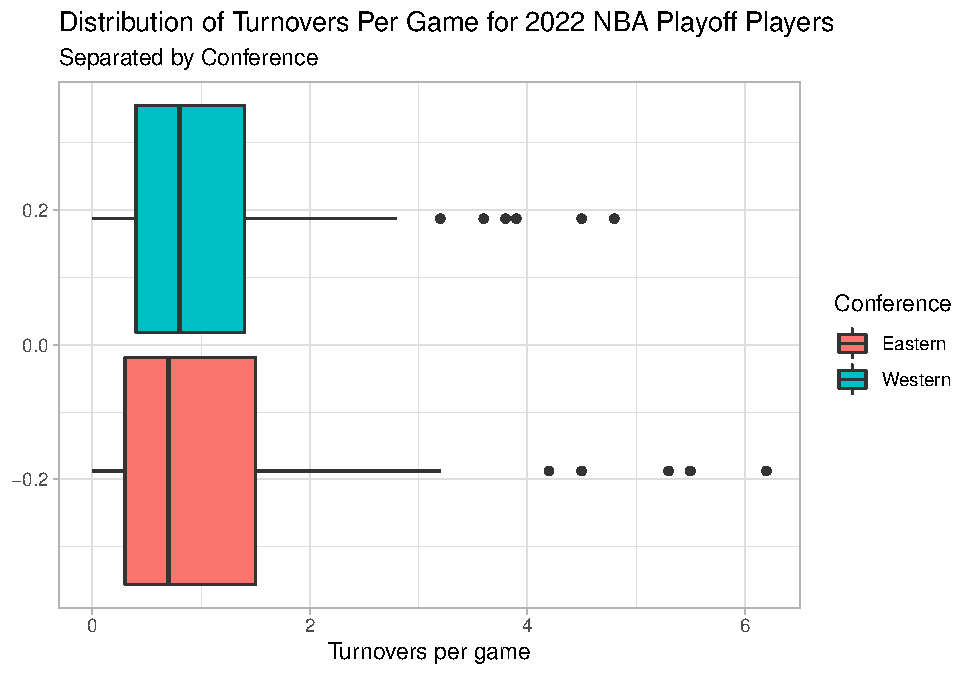
\includegraphics{Monday-Lab-Worksheet-Answers_files/figure-latex/unnamed-chunk-15-1.pdf}

\hypertarget{part-d}{%
\subsubsection{part d}\label{part-d}}

This is \emph{a} possible answer.

Overall, there is not that much of a difference. The Median for the
Western conference is higher, but the Eastern conference distribution is
a little more variable, but overall both distributions exhibit a right
skew and their medians are relatively close to one another.

\hypertarget{part-e}{%
\subsubsection{part e}\label{part-e}}

Here is \emph{a} possible solution (code-wise).

\begin{Shaded}
\begin{Highlighting}[]
\NormalTok{NBA\_3 }\SpecialCharTok{\%\textgreater{}\%} \FunctionTok{mutate}\NormalTok{(}\StringTok{\textasciigrave{}}\AttributeTok{eFG\%}\StringTok{\textasciigrave{}} \OtherTok{=} \FunctionTok{as.numeric}\NormalTok{(}\StringTok{\textasciigrave{}}\AttributeTok{eFG\%}\StringTok{\textasciigrave{}}\NormalTok{)) }\SpecialCharTok{\%\textgreater{}\%}  \FunctionTok{group\_by}\NormalTok{(Conference) }\SpecialCharTok{\%\textgreater{}\%} 
  \FunctionTok{summarise}\NormalTok{(}\AttributeTok{Mean =} \FunctionTok{mean}\NormalTok{(}\StringTok{\textasciigrave{}}\AttributeTok{eFG\%}\StringTok{\textasciigrave{}}\NormalTok{), }\AttributeTok{Median =} \FunctionTok{median}\NormalTok{(}\StringTok{\textasciigrave{}}\AttributeTok{eFG\%}\StringTok{\textasciigrave{}}\NormalTok{),}
            \AttributeTok{IQR =} \FunctionTok{IQR}\NormalTok{(}\StringTok{\textasciigrave{}}\AttributeTok{eFG\%}\StringTok{\textasciigrave{}}\NormalTok{), }\AttributeTok{SD =} \FunctionTok{sd}\NormalTok{(}\StringTok{\textasciigrave{}}\AttributeTok{eFG\%}\StringTok{\textasciigrave{}}\NormalTok{), }\AttributeTok{MAD =} \FunctionTok{mad}\NormalTok{(}\StringTok{\textasciigrave{}}\AttributeTok{eFG\%}\StringTok{\textasciigrave{}}\NormalTok{))}
\end{Highlighting}
\end{Shaded}

\begin{verbatim}
## # A tibble: 2 x 6
##   Conference  Mean Median    IQR     SD    MAD
##   <chr>      <dbl>  <dbl>  <dbl>  <dbl>  <dbl>
## 1 Eastern    0.521  0.516 0.0725 0.0824 0.0630
## 2 Western    0.523  0.525 0.078  0.0672 0.0578
\end{verbatim}

\begin{Shaded}
\begin{Highlighting}[]
\NormalTok{NBA\_3 }\SpecialCharTok{\%\textgreater{}\%} \FunctionTok{mutate}\NormalTok{(}\StringTok{\textasciigrave{}}\AttributeTok{eFG\%}\StringTok{\textasciigrave{}} \OtherTok{=} \FunctionTok{as.numeric}\NormalTok{(}\StringTok{\textasciigrave{}}\AttributeTok{eFG\%}\StringTok{\textasciigrave{}}\NormalTok{)) }\SpecialCharTok{\%\textgreater{}\%} 
  \FunctionTok{ggplot}\NormalTok{() }\SpecialCharTok{+} \FunctionTok{geom\_boxplot}\NormalTok{(}\AttributeTok{mapping =} \FunctionTok{aes}\NormalTok{(}\AttributeTok{x =} \StringTok{\textasciigrave{}}\AttributeTok{eFG\%}\StringTok{\textasciigrave{}}\NormalTok{, }\AttributeTok{fill =}\NormalTok{ Conference)) }\SpecialCharTok{+}
  \FunctionTok{ggtitle}\NormalTok{(}\StringTok{"Distribution of EFG Pct per game for 2022 NBA Playoff Players"}\NormalTok{,}
          \AttributeTok{subtitle =} \StringTok{"Separated by Conference"}\NormalTok{) }\SpecialCharTok{+} \FunctionTok{xlab}\NormalTok{(}\StringTok{"EFG Pct per game "}\NormalTok{) }\SpecialCharTok{+} \FunctionTok{theme\_light}\NormalTok{()}
\end{Highlighting}
\end{Shaded}

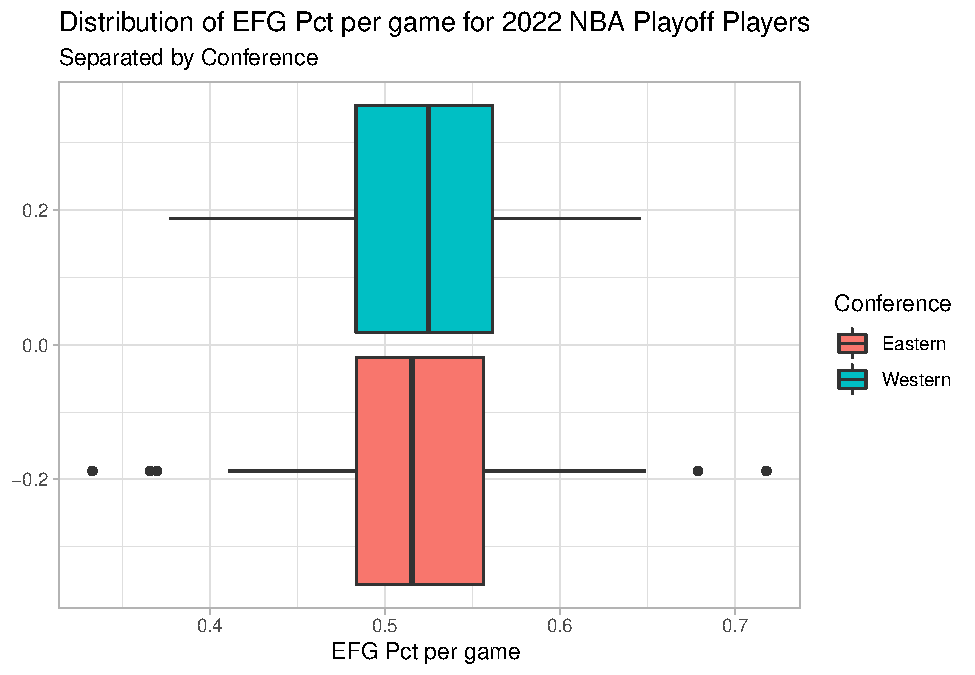
\includegraphics{Monday-Lab-Worksheet-Answers_files/figure-latex/unnamed-chunk-17-1.pdf}

This is \emph{a} possible answer to the written portion.

We see that the variability in the two distributions is pretty similar,
save for some outliers in the Eastern conference on both sides. However,
it looks like the median eFG\% is larger in the Western Conference. This
might suggest that the Western Conference is a \emph{slightly} better
conference when it comes to shooters.

\hypertarget{week-3---roulette}{%
\subsection{(Week 3) - Roulette}\label{week-3---roulette}}

\hypertarget{part-a-1}{%
\subsubsection{part a}\label{part-a-1}}

I would create a random variable \(X\) that takes two outcomes: \(1\)
and \(-1\), with probabilities 18/38 and 20/38, respectively. Note that
it does not matter which color you choose; the probabilities remain the
same.

\hypertarget{part-b.}{%
\subsubsection{part b.}\label{part-b.}}

The Expected Value is given by
\[ \mathbb{E}(X) = [1 \cdot P(X=1)] + [-1 \cdot P(X = -1)]  = \frac{18}{38} - \frac{20}{38} = -\frac{2}{38} \approx -5 \space cents\].

The Variance (using the Computational Formula):

\[ Var(X) = \mathbb{E}(X^2) - (\mathbb{E}(X))^2 \] and we have that
since \(X\) takes either -1 or 1, squaring it means that \(X^2\) will
always take the value of 1. Hence we have the following calcuation of
\(\mathbb{E}{X^2}\):

\[ \mathbb{E}(X^2) = [1 \cdot P(X^2=1)] + [1 \cdot P(X^2 = 1)] = 1\]

so that

\$\$ Var(X) = \mathbb{E}(X\^{}2)

\begin{itemize}
\tightlist
\item
  (\mathbb{E}(X))\^{}2 = 1 - (-\frac{2}{38})\^{}2 = 1 - \frac{4}{38^2}
  \approx 0.997 \space dollars\^{}2\$\$
\end{itemize}

\hypertarget{part-c-1}{%
\subsubsection{part c}\label{part-c-1}}

\textbf{Note:} We are not playing 100 times, just merely playing once
with a larger bet (How would the calculation change if the former was
the case?).

Let's use some of the rules for expected value and variance. Let
\(a = 100\) be a constant. Then we have that

\[ \mathbb{E}(aX) =  a\cdot \mathbb{E}(X) = 100 \cdot \mathbb{E}(X)
\approx -500 \space cents = -5 \space dollars\].

\[ Var(aX) =  a^2\cdot Var(X) = 1000 \cdot Var(X)
\approx 1003 \space dollars^2\].

\hypertarget{week-3---penguins}{%
\subsection{(Week 3) - Penguins}\label{week-3---penguins}}

Choice \emph{a.} and choice \emph{c.} are examples of generalizations.

\hypertarget{week-2---penguins}{%
\subsection{(Week 2) - Penguins}\label{week-2---penguins}}

First plot:

\begin{Shaded}
\begin{Highlighting}[]
\NormalTok{p2 }\OtherTok{\textless{}{-}} \FunctionTok{ggplot}\NormalTok{(penguins, }
             \FunctionTok{aes}\NormalTok{(}\AttributeTok{x =}\NormalTok{ species)) }\SpecialCharTok{+}
  \FunctionTok{geom\_bar}\NormalTok{() }\SpecialCharTok{+}
  \FunctionTok{xlab}\NormalTok{(}\StringTok{"Species"}\NormalTok{) }\SpecialCharTok{+} \FunctionTok{ylab}\NormalTok{(}\StringTok{"Count"}\NormalTok{) }\SpecialCharTok{+} 
      \FunctionTok{theme\_gray}\NormalTok{(}\AttributeTok{base\_size =} \DecValTok{8}\NormalTok{)}
\end{Highlighting}
\end{Shaded}

Second plot:

\begin{Shaded}
\begin{Highlighting}[]
\NormalTok{p3 }\OtherTok{\textless{}{-}} \FunctionTok{ggplot}\NormalTok{(penguins,}
             \FunctionTok{aes}\NormalTok{(}\AttributeTok{x =}\NormalTok{ flipper\_length\_mm,}
                 \AttributeTok{y =}\NormalTok{ body\_mass\_g,}
                 \AttributeTok{color =}\NormalTok{ island)) }\SpecialCharTok{+}
  \FunctionTok{geom\_point}\NormalTok{() }\SpecialCharTok{+} \FunctionTok{xlab}\NormalTok{(}\StringTok{"Flipper Length"}\NormalTok{) }\SpecialCharTok{+} \FunctionTok{ylab}\NormalTok{(}\StringTok{"Body Mass"}\NormalTok{) }\SpecialCharTok{+} 
      \FunctionTok{theme\_gray}\NormalTok{(}\AttributeTok{base\_size =} \DecValTok{8}\NormalTok{)}
\end{Highlighting}
\end{Shaded}

\hypertarget{week-2---flights}{%
\subsection{(Week 2) - Flights}\label{week-2---flights}}

\begin{Shaded}
\begin{Highlighting}[]
\NormalTok{flights }\SpecialCharTok{\%\textgreater{}\%}
  \FunctionTok{ggplot}\NormalTok{(}\FunctionTok{aes}\NormalTok{(}\AttributeTok{x =}\NormalTok{ dep\_delay)) }\SpecialCharTok{+} 
  \FunctionTok{geom\_histogram}\NormalTok{(}\AttributeTok{binwidth =} \DecValTok{15}\NormalTok{) }\SpecialCharTok{+}
  \FunctionTok{xlim}\NormalTok{(}\FunctionTok{c}\NormalTok{(}\SpecialCharTok{{-}}\DecValTok{50}\NormalTok{, }\DecValTok{100}\NormalTok{))}
\NormalTok{flights }\SpecialCharTok{\%\textgreater{}\%}
  \FunctionTok{summarise}\NormalTok{(}\AttributeTok{med\_delay =} \FunctionTok{median}\NormalTok{(dep\_delay, }\AttributeTok{na.rm =}\NormalTok{ T),}
            \AttributeTok{iqr\_delay =} \FunctionTok{IQR}\NormalTok{(dep\_delay, }\AttributeTok{na.rm =}\NormalTok{ T))}
\end{Highlighting}
\end{Shaded}

The statistical summaries should be median and IQR since we have a
skewed distribution. The shape students should describe as unimodal and
right skewed.

\hypertarget{week-3---distributions}{%
\subsection{(Week 3) - Distributions}\label{week-3---distributions}}

The answer is \(X \sim Binomial(n = 8, p =.8)\)

\end{document}
